% Created by tikzDevice version 0.7.0 on 2014-07-26 02:55:27
% !TEX encoding = UTF-8 Unicode
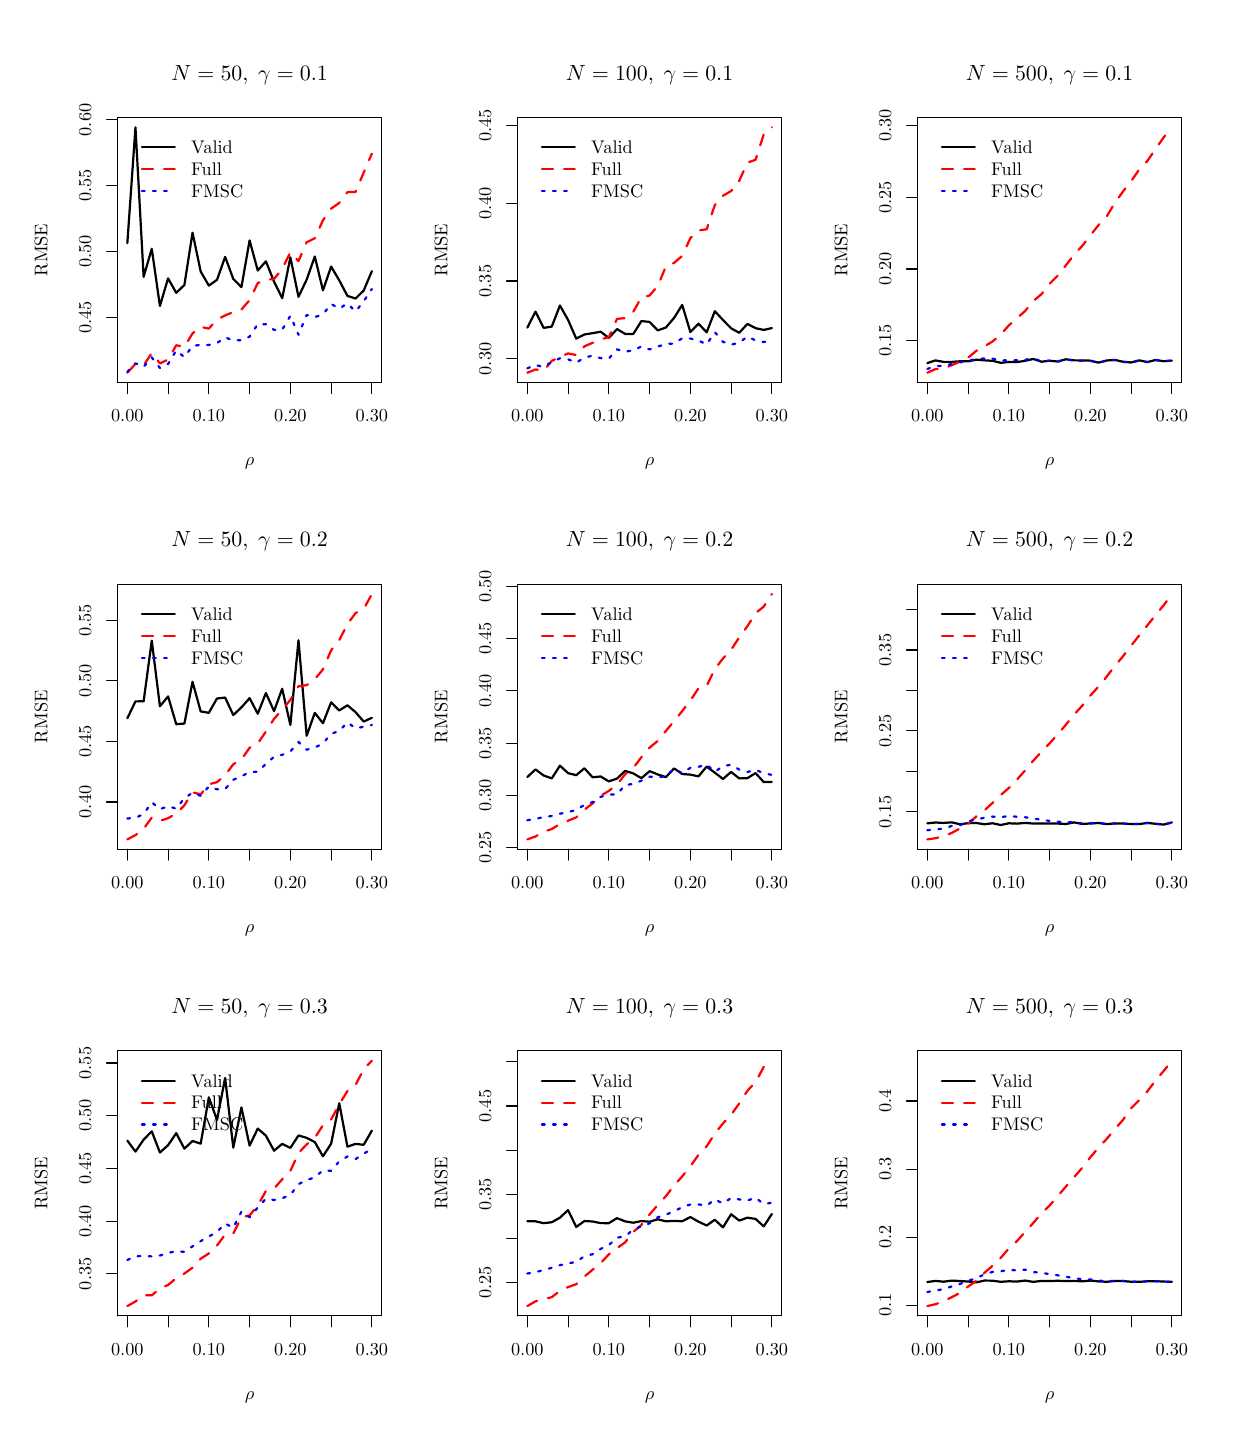
\begin{tikzpicture}[x=1pt,y=1pt]
\definecolor[named]{fillColor}{rgb}{1.00,1.00,1.00}
\path[use as bounding box,fill=fillColor,fill opacity=0.00] (0,0) rectangle (433.62,505.89);
\begin{scope}
\path[clip] ( 32.47,377.65) rectangle (127.91,473.42);
\definecolor[named]{drawColor}{rgb}{0.00,0.00,0.00}

\path[draw=drawColor,line width= 0.8pt,line join=round,line cap=round] ( 36.01,428.00) --
	( 38.95,469.87) --
	( 41.90,415.85) --
	( 44.84,425.99) --
	( 47.79,405.33) --
	( 50.73,415.30) --
	( 53.68,410.08) --
	( 56.63,412.90) --
	( 59.57,431.80) --
	( 62.52,417.77) --
	( 65.46,412.69) --
	( 68.41,414.75) --
	( 71.35,423.06) --
	( 74.30,415.09) --
	( 77.24,412.13) --
	( 80.19,429.01) --
	( 83.14,418.14) --
	( 86.08,421.45) --
	( 89.03,414.08) --
	( 91.97,408.14) --
	( 94.92,422.89) --
	( 97.86,408.65) --
	(100.81,414.84) --
	(103.75,423.19) --
	(106.70,410.98) --
	(109.65,419.56) --
	(112.59,414.59) --
	(115.54,408.96) --
	(118.48,408.00) --
	(121.43,410.92) --
	(124.37,417.89);
\end{scope}
\begin{scope}
\path[clip] (  0.00,  0.00) rectangle (433.62,505.89);
\definecolor[named]{drawColor}{rgb}{0.00,0.00,0.00}

\path[draw=drawColor,line width= 0.4pt,line join=round,line cap=round] ( 36.01,377.65) -- (124.37,377.65);

\path[draw=drawColor,line width= 0.4pt,line join=round,line cap=round] ( 36.01,377.65) -- ( 36.01,373.69);

\path[draw=drawColor,line width= 0.4pt,line join=round,line cap=round] ( 50.73,377.65) -- ( 50.73,373.69);

\path[draw=drawColor,line width= 0.4pt,line join=round,line cap=round] ( 65.46,377.65) -- ( 65.46,373.69);

\path[draw=drawColor,line width= 0.4pt,line join=round,line cap=round] ( 80.19,377.65) -- ( 80.19,373.69);

\path[draw=drawColor,line width= 0.4pt,line join=round,line cap=round] ( 94.92,377.65) -- ( 94.92,373.69);

\path[draw=drawColor,line width= 0.4pt,line join=round,line cap=round] (109.65,377.65) -- (109.65,373.69);

\path[draw=drawColor,line width= 0.4pt,line join=round,line cap=round] (124.37,377.65) -- (124.37,373.69);

\node[text=drawColor,anchor=base,inner sep=0pt, outer sep=0pt, scale=  0.66] at ( 36.01,363.40) {0.00};

\node[text=drawColor,anchor=base,inner sep=0pt, outer sep=0pt, scale=  0.66] at ( 65.46,363.40) {0.10};

\node[text=drawColor,anchor=base,inner sep=0pt, outer sep=0pt, scale=  0.66] at ( 94.92,363.40) {0.20};

\node[text=drawColor,anchor=base,inner sep=0pt, outer sep=0pt, scale=  0.66] at (124.37,363.40) {0.30};

\path[draw=drawColor,line width= 0.4pt,line join=round,line cap=round] ( 32.47,401.28) -- ( 32.47,472.56);

\path[draw=drawColor,line width= 0.4pt,line join=round,line cap=round] ( 32.47,401.28) -- ( 28.51,401.28);

\path[draw=drawColor,line width= 0.4pt,line join=round,line cap=round] ( 32.47,425.04) -- ( 28.51,425.04);

\path[draw=drawColor,line width= 0.4pt,line join=round,line cap=round] ( 32.47,448.80) -- ( 28.51,448.80);

\path[draw=drawColor,line width= 0.4pt,line join=round,line cap=round] ( 32.47,472.56) -- ( 28.51,472.56);

\node[text=drawColor,rotate= 90.00,anchor=base,inner sep=0pt, outer sep=0pt, scale=  0.66] at ( 22.97,401.28) {0.45};

\node[text=drawColor,rotate= 90.00,anchor=base,inner sep=0pt, outer sep=0pt, scale=  0.66] at ( 22.97,425.04) {0.50};

\node[text=drawColor,rotate= 90.00,anchor=base,inner sep=0pt, outer sep=0pt, scale=  0.66] at ( 22.97,448.80) {0.55};

\node[text=drawColor,rotate= 90.00,anchor=base,inner sep=0pt, outer sep=0pt, scale=  0.66] at ( 22.97,472.56) {0.60};

\path[draw=drawColor,line width= 0.4pt,line join=round,line cap=round] ( 32.47,377.65) --
	(127.91,377.65) --
	(127.91,473.42) --
	( 32.47,473.42) --
	( 32.47,377.65);
\end{scope}
\begin{scope}
\path[clip] (  0.00,337.26) rectangle (144.54,505.89);
\definecolor[named]{drawColor}{rgb}{0.00,0.00,0.00}

\node[text=drawColor,anchor=base,inner sep=0pt, outer sep=0pt, scale=  0.79] at ( 80.19,486.92) {\bfseries $N=50, \;\gamma=0.1$};

\node[text=drawColor,anchor=base,inner sep=0pt, outer sep=0pt, scale=  0.66] at ( 80.19,347.56) {$\rho$};

\node[text=drawColor,rotate= 90.00,anchor=base,inner sep=0pt, outer sep=0pt, scale=  0.66] at (  7.13,425.53) {RMSE};
\end{scope}
\begin{scope}
\path[clip] ( 32.47,377.65) rectangle (127.91,473.42);
\definecolor[named]{drawColor}{rgb}{1.00,0.00,0.00}

\path[draw=drawColor,line width= 0.8pt,dash pattern=on 4pt off 4pt ,line join=round,line cap=round] ( 36.01,381.20) --
	( 38.95,384.37) --
	( 41.90,383.86) --
	( 44.84,388.28) --
	( 47.79,384.57) --
	( 50.73,385.95) --
	( 53.68,391.12) --
	( 56.63,390.60) --
	( 59.57,395.41) --
	( 62.52,397.78) --
	( 65.46,397.14) --
	( 68.41,400.41) --
	( 71.35,401.91) --
	( 74.30,403.12) --
	( 77.24,404.04) --
	( 80.19,407.45) --
	( 83.14,413.60) --
	( 86.08,414.80) --
	( 89.03,415.09) --
	( 91.97,418.68) --
	( 94.92,424.74) --
	( 97.86,421.55) --
	(100.81,428.33) --
	(103.75,429.80) --
	(106.70,436.28) --
	(109.65,440.49) --
	(112.59,442.56) --
	(115.54,446.46) --
	(118.48,446.51) --
	(121.43,453.57) --
	(124.37,460.38);
\definecolor[named]{drawColor}{rgb}{0.00,0.00,1.00}

\path[draw=drawColor,line width= 0.8pt,dash pattern=on 1pt off 3pt ,line join=round,line cap=round] ( 36.01,381.47) --
	( 38.95,384.61) --
	( 41.90,383.30) --
	( 44.84,386.74) --
	( 47.79,382.90) --
	( 50.73,384.36) --
	( 53.68,389.24) --
	( 56.63,386.83) --
	( 59.57,390.89) --
	( 62.52,391.28) --
	( 65.46,391.25) --
	( 68.41,391.90) --
	( 71.35,393.98) --
	( 74.30,392.83) --
	( 77.24,392.99) --
	( 80.19,394.22) --
	( 83.14,398.80) --
	( 86.08,398.72) --
	( 89.03,396.68) --
	( 91.97,396.72) --
	( 94.92,401.78) --
	( 97.86,394.93) --
	(100.81,402.09) --
	(103.75,401.29) --
	(106.70,402.31) --
	(109.65,406.05) --
	(112.59,404.37) --
	(115.54,406.25) --
	(118.48,403.30) --
	(121.43,407.06) --
	(124.37,411.45);
\definecolor[named]{drawColor}{rgb}{0.00,0.00,0.00}

\path[draw=drawColor,line width= 0.8pt,line join=round,line cap=round] ( 41.28,462.63) -- ( 53.16,462.63);
\definecolor[named]{drawColor}{rgb}{1.00,0.00,0.00}

\path[draw=drawColor,line width= 0.8pt,dash pattern=on 4pt off 4pt ,line join=round,line cap=round] ( 41.28,454.71) -- ( 53.16,454.71);
\definecolor[named]{drawColor}{rgb}{0.00,0.00,1.00}

\path[draw=drawColor,line width= 0.8pt,dash pattern=on 1pt off 3pt ,line join=round,line cap=round] ( 41.28,446.79) -- ( 53.16,446.79);
\definecolor[named]{drawColor}{rgb}{0.00,0.00,0.00}

\node[text=drawColor,anchor=base west,inner sep=0pt, outer sep=0pt, scale=  0.66] at ( 59.10,460.35) {Valid};

\node[text=drawColor,anchor=base west,inner sep=0pt, outer sep=0pt, scale=  0.66] at ( 59.10,452.43) {Full};

\node[text=drawColor,anchor=base west,inner sep=0pt, outer sep=0pt, scale=  0.66] at ( 59.10,444.51) {FMSC};
\end{scope}
\begin{scope}
\path[clip] (177.01,377.65) rectangle (272.45,473.42);
\definecolor[named]{drawColor}{rgb}{0.00,0.00,0.00}

\path[draw=drawColor,line width= 0.8pt,line join=round,line cap=round] (180.55,397.49) --
	(183.49,403.27) --
	(186.44,397.40) --
	(189.38,397.87) --
	(192.33,405.50) --
	(195.27,400.29) --
	(198.22,393.53) --
	(201.17,395.01) --
	(204.11,395.49) --
	(207.06,396.01) --
	(210.00,393.77) --
	(212.95,396.98) --
	(215.89,395.23) --
	(218.84,395.21) --
	(221.78,399.88) --
	(224.73,399.55) --
	(227.68,396.50) --
	(230.62,397.53) --
	(233.57,401.01) --
	(236.51,405.70) --
	(239.46,395.91) --
	(242.40,398.90) --
	(245.35,395.81) --
	(248.29,403.43) --
	(251.24,400.26) --
	(254.19,397.25) --
	(257.13,395.63) --
	(260.08,398.85) --
	(263.02,397.30) --
	(265.97,396.67) --
	(268.91,397.33);
\end{scope}
\begin{scope}
\path[clip] (  0.00,  0.00) rectangle (433.62,505.89);
\definecolor[named]{drawColor}{rgb}{0.00,0.00,0.00}

\path[draw=drawColor,line width= 0.4pt,line join=round,line cap=round] (180.55,377.65) -- (268.91,377.65);

\path[draw=drawColor,line width= 0.4pt,line join=round,line cap=round] (180.55,377.65) -- (180.55,373.69);

\path[draw=drawColor,line width= 0.4pt,line join=round,line cap=round] (195.27,377.65) -- (195.27,373.69);

\path[draw=drawColor,line width= 0.4pt,line join=round,line cap=round] (210.00,377.65) -- (210.00,373.69);

\path[draw=drawColor,line width= 0.4pt,line join=round,line cap=round] (224.73,377.65) -- (224.73,373.69);

\path[draw=drawColor,line width= 0.4pt,line join=round,line cap=round] (239.46,377.65) -- (239.46,373.69);

\path[draw=drawColor,line width= 0.4pt,line join=round,line cap=round] (254.19,377.65) -- (254.19,373.69);

\path[draw=drawColor,line width= 0.4pt,line join=round,line cap=round] (268.91,377.65) -- (268.91,373.69);

\node[text=drawColor,anchor=base,inner sep=0pt, outer sep=0pt, scale=  0.66] at (180.55,363.40) {0.00};

\node[text=drawColor,anchor=base,inner sep=0pt, outer sep=0pt, scale=  0.66] at (210.00,363.40) {0.10};

\node[text=drawColor,anchor=base,inner sep=0pt, outer sep=0pt, scale=  0.66] at (239.46,363.40) {0.20};

\node[text=drawColor,anchor=base,inner sep=0pt, outer sep=0pt, scale=  0.66] at (268.91,363.40) {0.30};

\path[draw=drawColor,line width= 0.4pt,line join=round,line cap=round] (177.01,386.20) -- (177.01,470.63);

\path[draw=drawColor,line width= 0.4pt,line join=round,line cap=round] (177.01,386.20) -- (173.05,386.20);

\path[draw=drawColor,line width= 0.4pt,line join=round,line cap=round] (177.01,414.34) -- (173.05,414.34);

\path[draw=drawColor,line width= 0.4pt,line join=round,line cap=round] (177.01,442.48) -- (173.05,442.48);

\path[draw=drawColor,line width= 0.4pt,line join=round,line cap=round] (177.01,470.63) -- (173.05,470.63);

\node[text=drawColor,rotate= 90.00,anchor=base,inner sep=0pt, outer sep=0pt, scale=  0.66] at (167.51,386.20) {0.30};

\node[text=drawColor,rotate= 90.00,anchor=base,inner sep=0pt, outer sep=0pt, scale=  0.66] at (167.51,414.34) {0.35};

\node[text=drawColor,rotate= 90.00,anchor=base,inner sep=0pt, outer sep=0pt, scale=  0.66] at (167.51,442.48) {0.40};

\node[text=drawColor,rotate= 90.00,anchor=base,inner sep=0pt, outer sep=0pt, scale=  0.66] at (167.51,470.63) {0.45};

\path[draw=drawColor,line width= 0.4pt,line join=round,line cap=round] (177.01,377.65) --
	(272.45,377.65) --
	(272.45,473.42) --
	(177.01,473.42) --
	(177.01,377.65);
\end{scope}
\begin{scope}
\path[clip] (144.54,337.26) rectangle (289.08,505.89);
\definecolor[named]{drawColor}{rgb}{0.00,0.00,0.00}

\node[text=drawColor,anchor=base,inner sep=0pt, outer sep=0pt, scale=  0.79] at (224.73,486.92) {\bfseries $N=100, \;\gamma=0.1$};

\node[text=drawColor,anchor=base,inner sep=0pt, outer sep=0pt, scale=  0.66] at (224.73,347.56) {$\rho$};

\node[text=drawColor,rotate= 90.00,anchor=base,inner sep=0pt, outer sep=0pt, scale=  0.66] at (151.67,425.53) {RMSE};
\end{scope}
\begin{scope}
\path[clip] (177.01,377.65) rectangle (272.45,473.42);
\definecolor[named]{drawColor}{rgb}{1.00,0.00,0.00}

\path[draw=drawColor,line width= 0.8pt,dash pattern=on 4pt off 4pt ,line join=round,line cap=round] (180.55,381.20) --
	(183.49,382.38) --
	(186.44,381.94) --
	(189.38,385.47) --
	(192.33,386.92) --
	(195.27,388.18) --
	(198.22,387.58) --
	(201.17,390.75) --
	(204.11,391.99) --
	(207.06,393.25) --
	(210.00,394.01) --
	(212.95,400.66) --
	(215.89,400.94) --
	(218.84,403.25) --
	(221.78,408.46) --
	(224.73,409.11) --
	(227.68,412.57) --
	(230.62,419.62) --
	(233.57,420.89) --
	(236.51,423.42) --
	(239.46,429.84) --
	(242.40,432.61) --
	(245.35,433.04) --
	(248.29,441.76) --
	(251.24,445.13) --
	(254.19,446.88) --
	(257.13,450.59) --
	(260.08,457.14) --
	(263.02,458.14) --
	(265.97,467.32) --
	(268.91,469.87);
\definecolor[named]{drawColor}{rgb}{0.00,0.00,1.00}

\path[draw=drawColor,line width= 0.8pt,dash pattern=on 1pt off 3pt ,line join=round,line cap=round] (180.55,382.79) --
	(183.49,384.01) --
	(186.44,383.24) --
	(189.38,385.13) --
	(192.33,386.40) --
	(195.27,386.06) --
	(198.22,384.81) --
	(201.17,386.66) --
	(204.11,387.36) --
	(207.06,386.48) --
	(210.00,386.32) --
	(212.95,389.64) --
	(215.89,388.81) --
	(218.84,389.27) --
	(221.78,390.70) --
	(224.73,389.62) --
	(227.68,390.61) --
	(230.62,391.66) --
	(233.57,391.70) --
	(236.51,393.66) --
	(239.46,393.54) --
	(242.40,392.86) --
	(245.35,391.42) --
	(248.29,395.85) --
	(251.24,392.36) --
	(254.19,391.34) --
	(257.13,392.08) --
	(260.08,394.25) --
	(263.02,392.89) --
	(265.97,392.27) --
	(268.91,393.14);
\definecolor[named]{drawColor}{rgb}{0.00,0.00,0.00}

\path[draw=drawColor,line width= 0.8pt,line join=round,line cap=round] (185.82,462.63) -- (197.70,462.63);
\definecolor[named]{drawColor}{rgb}{1.00,0.00,0.00}

\path[draw=drawColor,line width= 0.8pt,dash pattern=on 4pt off 4pt ,line join=round,line cap=round] (185.82,454.71) -- (197.70,454.71);
\definecolor[named]{drawColor}{rgb}{0.00,0.00,1.00}

\path[draw=drawColor,line width= 0.8pt,dash pattern=on 1pt off 3pt ,line join=round,line cap=round] (185.82,446.79) -- (197.70,446.79);
\definecolor[named]{drawColor}{rgb}{0.00,0.00,0.00}

\node[text=drawColor,anchor=base west,inner sep=0pt, outer sep=0pt, scale=  0.66] at (203.64,460.35) {Valid};

\node[text=drawColor,anchor=base west,inner sep=0pt, outer sep=0pt, scale=  0.66] at (203.64,452.43) {Full};

\node[text=drawColor,anchor=base west,inner sep=0pt, outer sep=0pt, scale=  0.66] at (203.64,444.51) {FMSC};
\end{scope}
\begin{scope}
\path[clip] (321.55,377.65) rectangle (416.99,473.42);
\definecolor[named]{drawColor}{rgb}{0.00,0.00,0.00}

\path[draw=drawColor,line width= 0.8pt,line join=round,line cap=round] (325.09,384.68) --
	(328.03,385.65) --
	(330.98,385.12) --
	(333.92,385.11) --
	(336.87,385.34) --
	(339.81,385.32) --
	(342.76,385.90) --
	(345.71,385.68) --
	(348.65,385.50) --
	(351.60,384.79) --
	(354.54,385.07) --
	(357.49,385.04) --
	(360.43,385.51) --
	(363.38,386.17) --
	(366.32,385.18) --
	(369.27,385.53) --
	(372.22,385.26) --
	(375.16,386.06) --
	(378.11,385.67) --
	(381.05,385.64) --
	(384.00,385.57) --
	(386.94,384.85) --
	(389.89,385.61) --
	(392.83,385.84) --
	(395.78,385.17) --
	(398.73,384.91) --
	(401.67,385.67) --
	(404.62,385.06) --
	(407.56,385.80) --
	(410.51,385.36) --
	(413.45,385.59);
\end{scope}
\begin{scope}
\path[clip] (  0.00,  0.00) rectangle (433.62,505.89);
\definecolor[named]{drawColor}{rgb}{0.00,0.00,0.00}

\path[draw=drawColor,line width= 0.4pt,line join=round,line cap=round] (325.09,377.65) -- (413.45,377.65);

\path[draw=drawColor,line width= 0.4pt,line join=round,line cap=round] (325.09,377.65) -- (325.09,373.69);

\path[draw=drawColor,line width= 0.4pt,line join=round,line cap=round] (339.81,377.65) -- (339.81,373.69);

\path[draw=drawColor,line width= 0.4pt,line join=round,line cap=round] (354.54,377.65) -- (354.54,373.69);

\path[draw=drawColor,line width= 0.4pt,line join=round,line cap=round] (369.27,377.65) -- (369.27,373.69);

\path[draw=drawColor,line width= 0.4pt,line join=round,line cap=round] (384.00,377.65) -- (384.00,373.69);

\path[draw=drawColor,line width= 0.4pt,line join=round,line cap=round] (398.73,377.65) -- (398.73,373.69);

\path[draw=drawColor,line width= 0.4pt,line join=round,line cap=round] (413.45,377.65) -- (413.45,373.69);

\node[text=drawColor,anchor=base,inner sep=0pt, outer sep=0pt, scale=  0.66] at (325.09,363.40) {0.00};

\node[text=drawColor,anchor=base,inner sep=0pt, outer sep=0pt, scale=  0.66] at (354.54,363.40) {0.10};

\node[text=drawColor,anchor=base,inner sep=0pt, outer sep=0pt, scale=  0.66] at (384.00,363.40) {0.20};

\node[text=drawColor,anchor=base,inner sep=0pt, outer sep=0pt, scale=  0.66] at (413.45,363.40) {0.30};

\path[draw=drawColor,line width= 0.4pt,line join=round,line cap=round] (321.55,392.77) -- (321.55,470.56);

\path[draw=drawColor,line width= 0.4pt,line join=round,line cap=round] (321.55,392.77) -- (317.59,392.77);

\path[draw=drawColor,line width= 0.4pt,line join=round,line cap=round] (321.55,418.70) -- (317.59,418.70);

\path[draw=drawColor,line width= 0.4pt,line join=round,line cap=round] (321.55,444.63) -- (317.59,444.63);

\path[draw=drawColor,line width= 0.4pt,line join=round,line cap=round] (321.55,470.56) -- (317.59,470.56);

\node[text=drawColor,rotate= 90.00,anchor=base,inner sep=0pt, outer sep=0pt, scale=  0.66] at (312.05,392.77) {0.15};

\node[text=drawColor,rotate= 90.00,anchor=base,inner sep=0pt, outer sep=0pt, scale=  0.66] at (312.05,418.70) {0.20};

\node[text=drawColor,rotate= 90.00,anchor=base,inner sep=0pt, outer sep=0pt, scale=  0.66] at (312.05,444.63) {0.25};

\node[text=drawColor,rotate= 90.00,anchor=base,inner sep=0pt, outer sep=0pt, scale=  0.66] at (312.05,470.56) {0.30};

\path[draw=drawColor,line width= 0.4pt,line join=round,line cap=round] (321.55,377.65) --
	(416.99,377.65) --
	(416.99,473.42) --
	(321.55,473.42) --
	(321.55,377.65);
\end{scope}
\begin{scope}
\path[clip] (289.08,337.26) rectangle (433.62,505.89);
\definecolor[named]{drawColor}{rgb}{0.00,0.00,0.00}

\node[text=drawColor,anchor=base,inner sep=0pt, outer sep=0pt, scale=  0.79] at (369.27,486.92) {\bfseries $N=500, \;\gamma=0.1$};

\node[text=drawColor,anchor=base,inner sep=0pt, outer sep=0pt, scale=  0.66] at (369.27,347.56) {$\rho$};

\node[text=drawColor,rotate= 90.00,anchor=base,inner sep=0pt, outer sep=0pt, scale=  0.66] at (296.21,425.53) {RMSE};
\end{scope}
\begin{scope}
\path[clip] (321.55,377.65) rectangle (416.99,473.42);
\definecolor[named]{drawColor}{rgb}{1.00,0.00,0.00}

\path[draw=drawColor,line width= 0.8pt,dash pattern=on 4pt off 4pt ,line join=round,line cap=round] (325.09,381.20) --
	(328.03,382.51) --
	(330.98,382.81) --
	(333.92,383.93) --
	(336.87,385.21) --
	(339.81,386.60) --
	(342.76,389.10) --
	(345.71,390.72) --
	(348.65,392.49) --
	(351.60,394.97) --
	(354.54,398.31) --
	(357.49,400.91) --
	(360.43,403.52) --
	(363.38,407.11) --
	(366.32,409.59) --
	(369.27,413.34) --
	(372.22,416.28) --
	(375.16,420.02) --
	(378.11,423.86) --
	(381.05,427.00) --
	(384.00,430.88) --
	(386.94,434.53) --
	(389.89,437.66) --
	(392.83,442.56) --
	(395.78,446.66) --
	(398.73,450.43) --
	(401.67,454.67) --
	(404.62,457.76) --
	(407.56,462.05) --
	(410.51,466.28) --
	(413.45,469.87);
\definecolor[named]{drawColor}{rgb}{0.00,0.00,1.00}

\path[draw=drawColor,line width= 0.8pt,dash pattern=on 1pt off 3pt ,line join=round,line cap=round] (325.09,382.58) --
	(328.03,383.56) --
	(330.98,383.75) --
	(333.92,384.31) --
	(336.87,384.96) --
	(339.81,385.42) --
	(342.76,386.24) --
	(345.71,386.32) --
	(348.65,386.30) --
	(351.60,385.58) --
	(354.54,385.77) --
	(357.49,385.70) --
	(360.43,385.90) --
	(363.38,386.30) --
	(366.32,385.36) --
	(369.27,385.57) --
	(372.22,385.23) --
	(375.16,385.99) --
	(378.11,385.60) --
	(381.05,385.54) --
	(384.00,385.50) --
	(386.94,384.81) --
	(389.89,385.56) --
	(392.83,385.77) --
	(395.78,385.12) --
	(398.73,384.86) --
	(401.67,385.64) --
	(404.62,385.04) --
	(407.56,385.76) --
	(410.51,385.34) --
	(413.45,385.57);
\definecolor[named]{drawColor}{rgb}{0.00,0.00,0.00}

\path[draw=drawColor,line width= 0.8pt,line join=round,line cap=round] (330.36,462.63) -- (342.24,462.63);
\definecolor[named]{drawColor}{rgb}{1.00,0.00,0.00}

\path[draw=drawColor,line width= 0.8pt,dash pattern=on 4pt off 4pt ,line join=round,line cap=round] (330.36,454.71) -- (342.24,454.71);
\definecolor[named]{drawColor}{rgb}{0.00,0.00,1.00}

\path[draw=drawColor,line width= 0.8pt,dash pattern=on 1pt off 3pt ,line join=round,line cap=round] (330.36,446.79) -- (342.24,446.79);
\definecolor[named]{drawColor}{rgb}{0.00,0.00,0.00}

\node[text=drawColor,anchor=base west,inner sep=0pt, outer sep=0pt, scale=  0.66] at (348.18,460.35) {Valid};

\node[text=drawColor,anchor=base west,inner sep=0pt, outer sep=0pt, scale=  0.66] at (348.18,452.43) {Full};

\node[text=drawColor,anchor=base west,inner sep=0pt, outer sep=0pt, scale=  0.66] at (348.18,444.51) {FMSC};
\end{scope}
\begin{scope}
\path[clip] ( 32.47,209.02) rectangle (127.91,304.79);
\definecolor[named]{drawColor}{rgb}{0.00,0.00,0.00}

\path[draw=drawColor,line width= 0.8pt,line join=round,line cap=round] ( 36.01,256.34) --
	( 38.95,262.44) --
	( 41.90,262.47) --
	( 44.84,284.39) --
	( 47.79,260.67) --
	( 50.73,264.24) --
	( 53.68,254.20) --
	( 56.63,254.42) --
	( 59.57,269.50) --
	( 62.52,258.82) --
	( 65.46,258.31) --
	( 68.41,263.48) --
	( 71.35,263.82) --
	( 74.30,257.49) --
	( 77.24,260.27) --
	( 80.19,263.61) --
	( 83.14,257.98) --
	( 86.08,265.46) --
	( 89.03,258.93) --
	( 91.97,267.00) --
	( 94.92,253.93) --
	( 97.86,284.53) --
	(100.81,250.02) --
	(103.75,258.30) --
	(106.70,254.55) --
	(109.65,262.11) --
	(112.59,259.16) --
	(115.54,261.03) --
	(118.48,258.55) --
	(121.43,255.14) --
	(124.37,256.51);
\end{scope}
\begin{scope}
\path[clip] (  0.00,  0.00) rectangle (433.62,505.89);
\definecolor[named]{drawColor}{rgb}{0.00,0.00,0.00}

\path[draw=drawColor,line width= 0.4pt,line join=round,line cap=round] ( 36.01,209.02) -- (124.37,209.02);

\path[draw=drawColor,line width= 0.4pt,line join=round,line cap=round] ( 36.01,209.02) -- ( 36.01,205.06);

\path[draw=drawColor,line width= 0.4pt,line join=round,line cap=round] ( 50.73,209.02) -- ( 50.73,205.06);

\path[draw=drawColor,line width= 0.4pt,line join=round,line cap=round] ( 65.46,209.02) -- ( 65.46,205.06);

\path[draw=drawColor,line width= 0.4pt,line join=round,line cap=round] ( 80.19,209.02) -- ( 80.19,205.06);

\path[draw=drawColor,line width= 0.4pt,line join=round,line cap=round] ( 94.92,209.02) -- ( 94.92,205.06);

\path[draw=drawColor,line width= 0.4pt,line join=round,line cap=round] (109.65,209.02) -- (109.65,205.06);

\path[draw=drawColor,line width= 0.4pt,line join=round,line cap=round] (124.37,209.02) -- (124.37,205.06);

\node[text=drawColor,anchor=base,inner sep=0pt, outer sep=0pt, scale=  0.66] at ( 36.01,194.77) {0.00};

\node[text=drawColor,anchor=base,inner sep=0pt, outer sep=0pt, scale=  0.66] at ( 65.46,194.77) {0.10};

\node[text=drawColor,anchor=base,inner sep=0pt, outer sep=0pt, scale=  0.66] at ( 94.92,194.77) {0.20};

\node[text=drawColor,anchor=base,inner sep=0pt, outer sep=0pt, scale=  0.66] at (124.37,194.77) {0.30};

\path[draw=drawColor,line width= 0.4pt,line join=round,line cap=round] ( 32.47,226.10) -- ( 32.47,291.78);

\path[draw=drawColor,line width= 0.4pt,line join=round,line cap=round] ( 32.47,226.10) -- ( 28.51,226.10);

\path[draw=drawColor,line width= 0.4pt,line join=round,line cap=round] ( 32.47,247.99) -- ( 28.51,247.99);

\path[draw=drawColor,line width= 0.4pt,line join=round,line cap=round] ( 32.47,269.89) -- ( 28.51,269.89);

\path[draw=drawColor,line width= 0.4pt,line join=round,line cap=round] ( 32.47,291.78) -- ( 28.51,291.78);

\node[text=drawColor,rotate= 90.00,anchor=base,inner sep=0pt, outer sep=0pt, scale=  0.66] at ( 22.97,226.10) {0.40};

\node[text=drawColor,rotate= 90.00,anchor=base,inner sep=0pt, outer sep=0pt, scale=  0.66] at ( 22.97,247.99) {0.45};

\node[text=drawColor,rotate= 90.00,anchor=base,inner sep=0pt, outer sep=0pt, scale=  0.66] at ( 22.97,269.89) {0.50};

\node[text=drawColor,rotate= 90.00,anchor=base,inner sep=0pt, outer sep=0pt, scale=  0.66] at ( 22.97,291.78) {0.55};

\path[draw=drawColor,line width= 0.4pt,line join=round,line cap=round] ( 32.47,209.02) --
	(127.91,209.02) --
	(127.91,304.79) --
	( 32.47,304.79) --
	( 32.47,209.02);
\end{scope}
\begin{scope}
\path[clip] (  0.00,168.63) rectangle (144.54,337.26);
\definecolor[named]{drawColor}{rgb}{0.00,0.00,0.00}

\node[text=drawColor,anchor=base,inner sep=0pt, outer sep=0pt, scale=  0.79] at ( 80.19,318.29) {\bfseries $N=50, \;\gamma=0.2$};

\node[text=drawColor,anchor=base,inner sep=0pt, outer sep=0pt, scale=  0.66] at ( 80.19,178.93) {$\rho$};

\node[text=drawColor,rotate= 90.00,anchor=base,inner sep=0pt, outer sep=0pt, scale=  0.66] at (  7.13,256.90) {RMSE};
\end{scope}
\begin{scope}
\path[clip] ( 32.47,209.02) rectangle (127.91,304.79);
\definecolor[named]{drawColor}{rgb}{1.00,0.00,0.00}

\path[draw=drawColor,line width= 0.8pt,dash pattern=on 4pt off 4pt ,line join=round,line cap=round] ( 36.01,212.57) --
	( 38.95,214.11) --
	( 41.90,216.40) --
	( 44.84,220.47) --
	( 47.79,219.25) --
	( 50.73,220.23) --
	( 53.68,221.88) --
	( 56.63,224.90) --
	( 59.57,229.60) --
	( 62.52,228.83) --
	( 65.46,232.49) --
	( 68.41,233.25) --
	( 71.35,235.76) --
	( 74.30,239.72) --
	( 77.24,241.48) --
	( 80.19,245.67) --
	( 83.14,247.23) --
	( 86.08,251.53) --
	( 89.03,256.12) --
	( 91.97,259.45) --
	( 94.92,262.97) --
	( 97.86,267.92) --
	(100.81,268.31) --
	(103.75,270.46) --
	(106.70,274.01) --
	(109.65,280.90) --
	(112.59,284.58) --
	(115.54,290.36) --
	(118.48,294.35) --
	(121.43,295.80) --
	(124.37,301.24);
\definecolor[named]{drawColor}{rgb}{0.00,0.00,1.00}

\path[draw=drawColor,line width= 0.8pt,dash pattern=on 1pt off 3pt ,line join=round,line cap=round] ( 36.01,220.12) --
	( 38.95,220.35) --
	( 41.90,221.74) --
	( 44.84,226.00) --
	( 47.79,223.47) --
	( 50.73,224.60) --
	( 53.68,223.66) --
	( 56.63,227.48) --
	( 59.57,229.41) --
	( 62.52,228.33) --
	( 65.46,231.69) --
	( 68.41,230.67) --
	( 71.35,230.76) --
	( 74.30,234.11) --
	( 77.24,235.37) --
	( 80.19,236.90) --
	( 83.14,237.01) --
	( 86.08,239.82) --
	( 89.03,242.44) --
	( 91.97,243.14) --
	( 94.92,244.35) --
	( 97.86,247.76) --
	(100.81,244.98) --
	(103.75,245.78) --
	(106.70,247.21) --
	(109.65,250.79) --
	(112.59,251.69) --
	(115.54,254.91) --
	(118.48,252.66) --
	(121.43,253.30) --
	(124.37,253.91);
\definecolor[named]{drawColor}{rgb}{0.00,0.00,0.00}

\path[draw=drawColor,line width= 0.8pt,line join=round,line cap=round] ( 41.28,294.00) -- ( 53.16,294.00);
\definecolor[named]{drawColor}{rgb}{1.00,0.00,0.00}

\path[draw=drawColor,line width= 0.8pt,dash pattern=on 4pt off 4pt ,line join=round,line cap=round] ( 41.28,286.08) -- ( 53.16,286.08);
\definecolor[named]{drawColor}{rgb}{0.00,0.00,1.00}

\path[draw=drawColor,line width= 0.8pt,dash pattern=on 1pt off 3pt ,line join=round,line cap=round] ( 41.28,278.16) -- ( 53.16,278.16);
\definecolor[named]{drawColor}{rgb}{0.00,0.00,0.00}

\node[text=drawColor,anchor=base west,inner sep=0pt, outer sep=0pt, scale=  0.66] at ( 59.10,291.72) {Valid};

\node[text=drawColor,anchor=base west,inner sep=0pt, outer sep=0pt, scale=  0.66] at ( 59.10,283.80) {Full};

\node[text=drawColor,anchor=base west,inner sep=0pt, outer sep=0pt, scale=  0.66] at ( 59.10,275.88) {FMSC};
\end{scope}
\begin{scope}
\path[clip] (177.01,209.02) rectangle (272.45,304.79);
\definecolor[named]{drawColor}{rgb}{0.00,0.00,0.00}

\path[draw=drawColor,line width= 0.8pt,line join=round,line cap=round] (180.55,235.10) --
	(183.49,237.86) --
	(186.44,235.66) --
	(189.38,234.62) --
	(192.33,239.22) --
	(195.27,236.51) --
	(198.22,235.77) --
	(201.17,238.27) --
	(204.11,235.02) --
	(207.06,235.30) --
	(210.00,233.54) --
	(212.95,234.55) --
	(215.89,237.33) --
	(218.84,236.40) --
	(221.78,234.69) --
	(224.73,237.22) --
	(227.68,236.04) --
	(230.62,235.09) --
	(233.57,238.22) --
	(236.51,236.20) --
	(239.46,235.97) --
	(242.40,235.35) --
	(245.35,238.88) --
	(248.29,236.69) --
	(251.24,234.41) --
	(254.19,236.94) --
	(257.13,234.61) --
	(260.08,234.70) --
	(263.02,236.52) --
	(265.97,233.30) --
	(268.91,233.31);
\end{scope}
\begin{scope}
\path[clip] (  0.00,  0.00) rectangle (433.62,505.89);
\definecolor[named]{drawColor}{rgb}{0.00,0.00,0.00}

\path[draw=drawColor,line width= 0.4pt,line join=round,line cap=round] (180.55,209.02) -- (268.91,209.02);

\path[draw=drawColor,line width= 0.4pt,line join=round,line cap=round] (180.55,209.02) -- (180.55,205.06);

\path[draw=drawColor,line width= 0.4pt,line join=round,line cap=round] (195.27,209.02) -- (195.27,205.06);

\path[draw=drawColor,line width= 0.4pt,line join=round,line cap=round] (210.00,209.02) -- (210.00,205.06);

\path[draw=drawColor,line width= 0.4pt,line join=round,line cap=round] (224.73,209.02) -- (224.73,205.06);

\path[draw=drawColor,line width= 0.4pt,line join=round,line cap=round] (239.46,209.02) -- (239.46,205.06);

\path[draw=drawColor,line width= 0.4pt,line join=round,line cap=round] (254.19,209.02) -- (254.19,205.06);

\path[draw=drawColor,line width= 0.4pt,line join=round,line cap=round] (268.91,209.02) -- (268.91,205.06);

\node[text=drawColor,anchor=base,inner sep=0pt, outer sep=0pt, scale=  0.66] at (180.55,194.77) {0.00};

\node[text=drawColor,anchor=base,inner sep=0pt, outer sep=0pt, scale=  0.66] at (210.00,194.77) {0.10};

\node[text=drawColor,anchor=base,inner sep=0pt, outer sep=0pt, scale=  0.66] at (239.46,194.77) {0.20};

\node[text=drawColor,anchor=base,inner sep=0pt, outer sep=0pt, scale=  0.66] at (268.91,194.77) {0.30};

\path[draw=drawColor,line width= 0.4pt,line join=round,line cap=round] (177.01,209.60) -- (177.01,303.96);

\path[draw=drawColor,line width= 0.4pt,line join=round,line cap=round] (177.01,209.60) -- (173.05,209.60);

\path[draw=drawColor,line width= 0.4pt,line join=round,line cap=round] (177.01,228.48) -- (173.05,228.48);

\path[draw=drawColor,line width= 0.4pt,line join=round,line cap=round] (177.01,247.35) -- (173.05,247.35);

\path[draw=drawColor,line width= 0.4pt,line join=round,line cap=round] (177.01,266.22) -- (173.05,266.22);

\path[draw=drawColor,line width= 0.4pt,line join=round,line cap=round] (177.01,285.09) -- (173.05,285.09);

\path[draw=drawColor,line width= 0.4pt,line join=round,line cap=round] (177.01,303.96) -- (173.05,303.96);

\node[text=drawColor,rotate= 90.00,anchor=base,inner sep=0pt, outer sep=0pt, scale=  0.66] at (167.51,209.60) {0.25};

\node[text=drawColor,rotate= 90.00,anchor=base,inner sep=0pt, outer sep=0pt, scale=  0.66] at (167.51,228.48) {0.30};

\node[text=drawColor,rotate= 90.00,anchor=base,inner sep=0pt, outer sep=0pt, scale=  0.66] at (167.51,247.35) {0.35};

\node[text=drawColor,rotate= 90.00,anchor=base,inner sep=0pt, outer sep=0pt, scale=  0.66] at (167.51,266.22) {0.40};

\node[text=drawColor,rotate= 90.00,anchor=base,inner sep=0pt, outer sep=0pt, scale=  0.66] at (167.51,285.09) {0.45};

\node[text=drawColor,rotate= 90.00,anchor=base,inner sep=0pt, outer sep=0pt, scale=  0.66] at (167.51,303.96) {0.50};

\path[draw=drawColor,line width= 0.4pt,line join=round,line cap=round] (177.01,209.02) --
	(272.45,209.02) --
	(272.45,304.79) --
	(177.01,304.79) --
	(177.01,209.02);
\end{scope}
\begin{scope}
\path[clip] (144.54,168.63) rectangle (289.08,337.26);
\definecolor[named]{drawColor}{rgb}{0.00,0.00,0.00}

\node[text=drawColor,anchor=base,inner sep=0pt, outer sep=0pt, scale=  0.79] at (224.73,318.29) {\bfseries $N=100, \;\gamma=0.2$};

\node[text=drawColor,anchor=base,inner sep=0pt, outer sep=0pt, scale=  0.66] at (224.73,178.93) {$\rho$};

\node[text=drawColor,rotate= 90.00,anchor=base,inner sep=0pt, outer sep=0pt, scale=  0.66] at (151.67,256.90) {RMSE};
\end{scope}
\begin{scope}
\path[clip] (177.01,209.02) rectangle (272.45,304.79);
\definecolor[named]{drawColor}{rgb}{1.00,0.00,0.00}

\path[draw=drawColor,line width= 0.8pt,dash pattern=on 4pt off 4pt ,line join=round,line cap=round] (180.55,212.57) --
	(183.49,213.61) --
	(186.44,215.36) --
	(189.38,216.30) --
	(192.33,218.14) --
	(195.27,219.32) --
	(198.22,220.52) --
	(201.17,223.31) --
	(204.11,225.56) --
	(207.06,228.34) --
	(210.00,230.10) --
	(212.95,232.37) --
	(215.89,236.14) --
	(218.84,238.40) --
	(221.78,242.29) --
	(224.73,245.73) --
	(227.68,248.15) --
	(230.62,251.77) --
	(233.57,255.30) --
	(236.51,258.91) --
	(239.46,262.76) --
	(242.40,267.18) --
	(245.35,268.01) --
	(248.29,274.12) --
	(251.24,277.94) --
	(254.19,281.10) --
	(257.13,285.57) --
	(260.08,289.61) --
	(263.02,294.31) --
	(265.97,296.69) --
	(268.91,301.24);
\definecolor[named]{drawColor}{rgb}{0.00,0.00,1.00}

\path[draw=drawColor,line width= 0.8pt,dash pattern=on 1pt off 3pt ,line join=round,line cap=round] (180.55,219.48) --
	(183.49,220.00) --
	(186.44,220.60) --
	(189.38,221.03) --
	(192.33,221.85) --
	(195.27,222.43) --
	(198.22,223.22) --
	(201.17,225.04) --
	(204.11,226.01) --
	(207.06,227.94) --
	(210.00,228.78) --
	(212.95,228.81) --
	(215.89,232.25) --
	(218.84,232.60) --
	(221.78,233.79) --
	(224.73,235.23) --
	(227.68,235.06) --
	(230.62,235.28) --
	(233.57,238.06) --
	(236.51,236.47) --
	(239.46,238.42) --
	(242.40,238.80) --
	(245.35,239.61) --
	(248.29,236.99) --
	(251.24,239.05) --
	(254.19,239.55) --
	(257.13,237.79) --
	(260.08,236.92) --
	(263.02,237.69) --
	(265.97,236.48) --
	(268.91,235.88);
\definecolor[named]{drawColor}{rgb}{0.00,0.00,0.00}

\path[draw=drawColor,line width= 0.8pt,line join=round,line cap=round] (185.82,294.00) -- (197.70,294.00);
\definecolor[named]{drawColor}{rgb}{1.00,0.00,0.00}

\path[draw=drawColor,line width= 0.8pt,dash pattern=on 4pt off 4pt ,line join=round,line cap=round] (185.82,286.08) -- (197.70,286.08);
\definecolor[named]{drawColor}{rgb}{0.00,0.00,1.00}

\path[draw=drawColor,line width= 0.8pt,dash pattern=on 1pt off 3pt ,line join=round,line cap=round] (185.82,278.16) -- (197.70,278.16);
\definecolor[named]{drawColor}{rgb}{0.00,0.00,0.00}

\node[text=drawColor,anchor=base west,inner sep=0pt, outer sep=0pt, scale=  0.66] at (203.64,291.72) {Valid};

\node[text=drawColor,anchor=base west,inner sep=0pt, outer sep=0pt, scale=  0.66] at (203.64,283.80) {Full};

\node[text=drawColor,anchor=base west,inner sep=0pt, outer sep=0pt, scale=  0.66] at (203.64,275.88) {FMSC};
\end{scope}
\begin{scope}
\path[clip] (321.55,209.02) rectangle (416.99,304.79);
\definecolor[named]{drawColor}{rgb}{0.00,0.00,0.00}

\path[draw=drawColor,line width= 0.8pt,line join=round,line cap=round] (325.09,218.38) --
	(328.03,218.67) --
	(330.98,218.52) --
	(333.92,218.73) --
	(336.87,218.04) --
	(339.81,218.43) --
	(342.76,218.50) --
	(345.71,218.04) --
	(348.65,218.40) --
	(351.60,217.77) --
	(354.54,218.39) --
	(357.49,218.26) --
	(360.43,218.53) --
	(363.38,218.30) --
	(366.32,218.34) --
	(369.27,218.28) --
	(372.22,218.29) --
	(375.16,218.14) --
	(378.11,218.70) --
	(381.05,218.15) --
	(384.00,218.32) --
	(386.94,218.49) --
	(389.89,218.10) --
	(392.83,218.33) --
	(395.78,218.31) --
	(398.73,218.12) --
	(401.67,218.11) --
	(404.62,218.52) --
	(407.56,218.21) --
	(410.51,217.92) --
	(413.45,218.70);
\end{scope}
\begin{scope}
\path[clip] (  0.00,  0.00) rectangle (433.62,505.89);
\definecolor[named]{drawColor}{rgb}{0.00,0.00,0.00}

\path[draw=drawColor,line width= 0.4pt,line join=round,line cap=round] (325.09,209.02) -- (413.45,209.02);

\path[draw=drawColor,line width= 0.4pt,line join=round,line cap=round] (325.09,209.02) -- (325.09,205.06);

\path[draw=drawColor,line width= 0.4pt,line join=round,line cap=round] (339.81,209.02) -- (339.81,205.06);

\path[draw=drawColor,line width= 0.4pt,line join=round,line cap=round] (354.54,209.02) -- (354.54,205.06);

\path[draw=drawColor,line width= 0.4pt,line join=round,line cap=round] (369.27,209.02) -- (369.27,205.06);

\path[draw=drawColor,line width= 0.4pt,line join=round,line cap=round] (384.00,209.02) -- (384.00,205.06);

\path[draw=drawColor,line width= 0.4pt,line join=round,line cap=round] (398.73,209.02) -- (398.73,205.06);

\path[draw=drawColor,line width= 0.4pt,line join=round,line cap=round] (413.45,209.02) -- (413.45,205.06);

\node[text=drawColor,anchor=base,inner sep=0pt, outer sep=0pt, scale=  0.66] at (325.09,194.77) {0.00};

\node[text=drawColor,anchor=base,inner sep=0pt, outer sep=0pt, scale=  0.66] at (354.54,194.77) {0.10};

\node[text=drawColor,anchor=base,inner sep=0pt, outer sep=0pt, scale=  0.66] at (384.00,194.77) {0.20};

\node[text=drawColor,anchor=base,inner sep=0pt, outer sep=0pt, scale=  0.66] at (413.45,194.77) {0.30};

\path[draw=drawColor,line width= 0.4pt,line join=round,line cap=round] (321.55,222.53) -- (321.55,295.64);

\path[draw=drawColor,line width= 0.4pt,line join=round,line cap=round] (321.55,222.53) -- (317.59,222.53);

\path[draw=drawColor,line width= 0.4pt,line join=round,line cap=round] (321.55,237.15) -- (317.59,237.15);

\path[draw=drawColor,line width= 0.4pt,line join=round,line cap=round] (321.55,251.77) -- (317.59,251.77);

\path[draw=drawColor,line width= 0.4pt,line join=round,line cap=round] (321.55,266.40) -- (317.59,266.40);

\path[draw=drawColor,line width= 0.4pt,line join=round,line cap=round] (321.55,281.02) -- (317.59,281.02);

\path[draw=drawColor,line width= 0.4pt,line join=round,line cap=round] (321.55,295.64) -- (317.59,295.64);

\node[text=drawColor,rotate= 90.00,anchor=base,inner sep=0pt, outer sep=0pt, scale=  0.66] at (312.05,222.53) {0.15};

\node[text=drawColor,rotate= 90.00,anchor=base,inner sep=0pt, outer sep=0pt, scale=  0.66] at (312.05,251.77) {0.25};

\node[text=drawColor,rotate= 90.00,anchor=base,inner sep=0pt, outer sep=0pt, scale=  0.66] at (312.05,281.02) {0.35};

\path[draw=drawColor,line width= 0.4pt,line join=round,line cap=round] (321.55,209.02) --
	(416.99,209.02) --
	(416.99,304.79) --
	(321.55,304.79) --
	(321.55,209.02);
\end{scope}
\begin{scope}
\path[clip] (289.08,168.63) rectangle (433.62,337.26);
\definecolor[named]{drawColor}{rgb}{0.00,0.00,0.00}

\node[text=drawColor,anchor=base,inner sep=0pt, outer sep=0pt, scale=  0.79] at (369.27,318.29) {\bfseries $N=500, \;\gamma=0.2$};

\node[text=drawColor,anchor=base,inner sep=0pt, outer sep=0pt, scale=  0.66] at (369.27,178.93) {$\rho$};

\node[text=drawColor,rotate= 90.00,anchor=base,inner sep=0pt, outer sep=0pt, scale=  0.66] at (296.21,256.90) {RMSE};
\end{scope}
\begin{scope}
\path[clip] (321.55,209.02) rectangle (416.99,304.79);
\definecolor[named]{drawColor}{rgb}{1.00,0.00,0.00}

\path[draw=drawColor,line width= 0.8pt,dash pattern=on 4pt off 4pt ,line join=round,line cap=round] (325.09,212.57) --
	(328.03,212.99) --
	(330.98,213.76) --
	(333.92,214.91) --
	(336.87,216.51) --
	(339.81,218.27) --
	(342.76,220.84) --
	(345.71,223.05) --
	(348.65,225.75) --
	(351.60,228.57) --
	(354.54,231.15) --
	(357.49,234.20) --
	(360.43,237.52) --
	(363.38,241.02) --
	(366.32,244.21) --
	(369.27,247.27) --
	(372.22,250.57) --
	(375.16,254.03) --
	(378.11,257.63) --
	(381.05,260.87) --
	(384.00,264.58) --
	(386.94,267.78) --
	(389.89,271.38) --
	(392.83,275.25) --
	(395.78,278.72) --
	(398.73,282.62) --
	(401.67,286.29) --
	(404.62,289.93) --
	(407.56,293.64) --
	(410.51,297.19) --
	(413.45,301.24);
\definecolor[named]{drawColor}{rgb}{0.00,0.00,1.00}

\path[draw=drawColor,line width= 0.8pt,dash pattern=on 1pt off 3pt ,line join=round,line cap=round] (325.09,215.88) --
	(328.03,216.15) --
	(330.98,216.50) --
	(333.92,217.41) --
	(336.87,217.71) --
	(339.81,219.09) --
	(342.76,219.85) --
	(345.71,220.35) --
	(348.65,220.81) --
	(351.60,220.54) --
	(354.54,221.10) --
	(357.49,220.73) --
	(360.43,220.57) --
	(363.38,220.10) --
	(366.32,219.71) --
	(369.27,219.23) --
	(372.22,218.99) --
	(375.16,218.60) --
	(378.11,218.98) --
	(381.05,218.28) --
	(384.00,218.39) --
	(386.94,218.55) --
	(389.89,218.11) --
	(392.83,218.34) --
	(395.78,218.31) --
	(398.73,218.12) --
	(401.67,218.11) --
	(404.62,218.52) --
	(407.56,218.21) --
	(410.51,217.92) --
	(413.45,218.70);
\definecolor[named]{drawColor}{rgb}{0.00,0.00,0.00}

\path[draw=drawColor,line width= 0.8pt,line join=round,line cap=round] (330.36,294.00) -- (342.24,294.00);
\definecolor[named]{drawColor}{rgb}{1.00,0.00,0.00}

\path[draw=drawColor,line width= 0.8pt,dash pattern=on 4pt off 4pt ,line join=round,line cap=round] (330.36,286.08) -- (342.24,286.08);
\definecolor[named]{drawColor}{rgb}{0.00,0.00,1.00}

\path[draw=drawColor,line width= 0.8pt,dash pattern=on 1pt off 3pt ,line join=round,line cap=round] (330.36,278.16) -- (342.24,278.16);
\definecolor[named]{drawColor}{rgb}{0.00,0.00,0.00}

\node[text=drawColor,anchor=base west,inner sep=0pt, outer sep=0pt, scale=  0.66] at (348.18,291.72) {Valid};

\node[text=drawColor,anchor=base west,inner sep=0pt, outer sep=0pt, scale=  0.66] at (348.18,283.80) {Full};

\node[text=drawColor,anchor=base west,inner sep=0pt, outer sep=0pt, scale=  0.66] at (348.18,275.88) {FMSC};
\end{scope}
\begin{scope}
\path[clip] ( 32.47, 40.39) rectangle (127.91,136.16);
\definecolor[named]{drawColor}{rgb}{0.00,0.00,0.00}

\path[draw=drawColor,line width= 0.8pt,line join=round,line cap=round] ( 36.01,103.75) --
	( 38.95, 99.76) --
	( 41.90,104.08) --
	( 44.84,107.08) --
	( 47.79, 99.42) --
	( 50.73,102.06) --
	( 53.68,106.41) --
	( 56.63,100.82) --
	( 59.57,103.60) --
	( 62.52,102.62) --
	( 65.46,119.36) --
	( 68.41,111.21) --
	( 71.35,126.36) --
	( 74.30,101.20) --
	( 77.24,115.72) --
	( 80.19,101.93) --
	( 83.14,108.07) --
	( 86.08,105.52) --
	( 89.03,100.08) --
	( 91.97,102.55) --
	( 94.92,101.09) --
	( 97.86,105.59) --
	(100.81,104.73) --
	(103.75,103.20) --
	(106.70, 98.07) --
	(109.65,102.60) --
	(112.59,117.25) --
	(115.54,101.54) --
	(118.48,102.55) --
	(121.43,102.22) --
	(124.37,107.33);
\end{scope}
\begin{scope}
\path[clip] (  0.00,  0.00) rectangle (433.62,505.89);
\definecolor[named]{drawColor}{rgb}{0.00,0.00,0.00}

\path[draw=drawColor,line width= 0.4pt,line join=round,line cap=round] ( 36.01, 40.39) -- (124.37, 40.39);

\path[draw=drawColor,line width= 0.4pt,line join=round,line cap=round] ( 36.01, 40.39) -- ( 36.01, 36.43);

\path[draw=drawColor,line width= 0.4pt,line join=round,line cap=round] ( 50.73, 40.39) -- ( 50.73, 36.43);

\path[draw=drawColor,line width= 0.4pt,line join=round,line cap=round] ( 65.46, 40.39) -- ( 65.46, 36.43);

\path[draw=drawColor,line width= 0.4pt,line join=round,line cap=round] ( 80.19, 40.39) -- ( 80.19, 36.43);

\path[draw=drawColor,line width= 0.4pt,line join=round,line cap=round] ( 94.92, 40.39) -- ( 94.92, 36.43);

\path[draw=drawColor,line width= 0.4pt,line join=round,line cap=round] (109.65, 40.39) -- (109.65, 36.43);

\path[draw=drawColor,line width= 0.4pt,line join=round,line cap=round] (124.37, 40.39) -- (124.37, 36.43);

\node[text=drawColor,anchor=base,inner sep=0pt, outer sep=0pt, scale=  0.66] at ( 36.01, 26.14) {0.00};

\node[text=drawColor,anchor=base,inner sep=0pt, outer sep=0pt, scale=  0.66] at ( 65.46, 26.14) {0.10};

\node[text=drawColor,anchor=base,inner sep=0pt, outer sep=0pt, scale=  0.66] at ( 94.92, 26.14) {0.20};

\node[text=drawColor,anchor=base,inner sep=0pt, outer sep=0pt, scale=  0.66] at (124.37, 26.14) {0.30};

\path[draw=drawColor,line width= 0.4pt,line join=round,line cap=round] ( 32.47, 55.59) -- ( 32.47,131.78);

\path[draw=drawColor,line width= 0.4pt,line join=round,line cap=round] ( 32.47, 55.59) -- ( 28.51, 55.59);

\path[draw=drawColor,line width= 0.4pt,line join=round,line cap=round] ( 32.47, 74.64) -- ( 28.51, 74.64);

\path[draw=drawColor,line width= 0.4pt,line join=round,line cap=round] ( 32.47, 93.69) -- ( 28.51, 93.69);

\path[draw=drawColor,line width= 0.4pt,line join=round,line cap=round] ( 32.47,112.74) -- ( 28.51,112.74);

\path[draw=drawColor,line width= 0.4pt,line join=round,line cap=round] ( 32.47,131.78) -- ( 28.51,131.78);

\node[text=drawColor,rotate= 90.00,anchor=base,inner sep=0pt, outer sep=0pt, scale=  0.66] at ( 22.97, 55.59) {0.35};

\node[text=drawColor,rotate= 90.00,anchor=base,inner sep=0pt, outer sep=0pt, scale=  0.66] at ( 22.97, 74.64) {0.40};

\node[text=drawColor,rotate= 90.00,anchor=base,inner sep=0pt, outer sep=0pt, scale=  0.66] at ( 22.97, 93.69) {0.45};

\node[text=drawColor,rotate= 90.00,anchor=base,inner sep=0pt, outer sep=0pt, scale=  0.66] at ( 22.97,112.74) {0.50};

\node[text=drawColor,rotate= 90.00,anchor=base,inner sep=0pt, outer sep=0pt, scale=  0.66] at ( 22.97,131.78) {0.55};

\path[draw=drawColor,line width= 0.4pt,line join=round,line cap=round] ( 32.47, 40.39) --
	(127.91, 40.39) --
	(127.91,136.16) --
	( 32.47,136.16) --
	( 32.47, 40.39);
\end{scope}
\begin{scope}
\path[clip] (  0.00,  0.00) rectangle (144.54,168.63);
\definecolor[named]{drawColor}{rgb}{0.00,0.00,0.00}

\node[text=drawColor,anchor=base,inner sep=0pt, outer sep=0pt, scale=  0.79] at ( 80.19,149.66) {\bfseries $N=50, \;\gamma=0.3$};

\node[text=drawColor,anchor=base,inner sep=0pt, outer sep=0pt, scale=  0.66] at ( 80.19, 10.30) {$\rho$};

\node[text=drawColor,rotate= 90.00,anchor=base,inner sep=0pt, outer sep=0pt, scale=  0.66] at (  7.13, 88.27) {RMSE};
\end{scope}
\begin{scope}
\path[clip] ( 32.47, 40.39) rectangle (127.91,136.16);
\definecolor[named]{drawColor}{rgb}{1.00,0.00,0.00}

\path[draw=drawColor,line width= 0.8pt,dash pattern=on 4pt off 4pt ,line join=round,line cap=round] ( 36.01, 43.94) --
	( 38.95, 45.61) --
	( 41.90, 47.92) --
	( 44.84, 47.80) --
	( 47.79, 50.34) --
	( 50.73, 51.56) --
	( 53.68, 54.01) --
	( 56.63, 55.70) --
	( 59.57, 57.80) --
	( 62.52, 61.04) --
	( 65.46, 62.97) --
	( 68.41, 65.80) --
	( 71.35, 69.79) --
	( 74.30, 70.16) --
	( 77.24, 75.98) --
	( 80.19, 76.72) --
	( 83.14, 80.28) --
	( 86.08, 85.52) --
	( 89.03, 86.39) --
	( 91.97, 89.75) --
	( 94.92, 92.74) --
	( 97.86, 99.24) --
	(100.81,102.36) --
	(103.75,104.71) --
	(106.70,109.29) --
	(109.65,111.39) --
	(112.59,116.78) --
	(115.54,121.66) --
	(118.48,123.87) --
	(121.43,129.54) --
	(124.37,132.61);
\definecolor[named]{drawColor}{rgb}{0.00,0.00,1.00}

\path[draw=drawColor,line width= 0.8pt,dash pattern=on 1pt off 3pt ,line join=round,line cap=round] ( 36.01, 60.59) --
	( 38.95, 61.93) --
	( 41.90, 62.06) --
	( 44.84, 61.88) --
	( 47.79, 62.20) --
	( 50.73, 63.16) --
	( 53.68, 63.75) --
	( 56.63, 63.54) --
	( 59.57, 65.52) --
	( 62.52, 67.41) --
	( 65.46, 69.10) --
	( 68.41, 70.69) --
	( 71.35, 73.78) --
	( 74.30, 72.20) --
	( 77.24, 78.07) --
	( 80.19, 76.02) --
	( 83.14, 79.57) --
	( 86.08, 82.73) --
	( 89.03, 82.26) --
	( 91.97, 82.92) --
	( 94.92, 84.08) --
	( 97.86, 88.00) --
	(100.81, 89.48) --
	(103.75, 90.46) --
	(106.70, 93.01) --
	(109.65, 92.82) --
	(112.59, 96.24) --
	(115.54, 97.97) --
	(118.48, 97.06) --
	(121.43, 99.01) --
	(124.37,100.76);
\definecolor[named]{drawColor}{rgb}{0.00,0.00,0.00}

\path[draw=drawColor,line width= 0.8pt,line join=round,line cap=round] ( 41.28,125.37) -- ( 53.16,125.37);
\definecolor[named]{drawColor}{rgb}{1.00,0.00,0.00}

\path[draw=drawColor,line width= 0.8pt,dash pattern=on 4pt off 4pt ,line join=round,line cap=round] ( 41.28,117.45) -- ( 53.16,117.45);
\definecolor[named]{drawColor}{rgb}{0.00,0.00,1.00}

\path[draw=drawColor,line width= 0.8pt,dash pattern=on 1pt off 3pt ,line join=round,line cap=round] ( 41.28,109.53) -- ( 53.16,109.53);
\definecolor[named]{drawColor}{rgb}{0.00,0.00,0.00}

\node[text=drawColor,anchor=base west,inner sep=0pt, outer sep=0pt, scale=  0.66] at ( 59.10,123.09) {Valid};

\node[text=drawColor,anchor=base west,inner sep=0pt, outer sep=0pt, scale=  0.66] at ( 59.10,115.17) {Full};

\node[text=drawColor,anchor=base west,inner sep=0pt, outer sep=0pt, scale=  0.66] at ( 59.10,107.25) {FMSC};
\end{scope}
\begin{scope}
\path[clip] (177.01, 40.39) rectangle (272.45,136.16);
\definecolor[named]{drawColor}{rgb}{0.00,0.00,0.00}

\path[draw=drawColor,line width= 0.8pt,line join=round,line cap=round] (180.55, 74.62) --
	(183.49, 74.56) --
	(186.44, 73.90) --
	(189.38, 74.23) --
	(192.33, 75.88) --
	(195.27, 78.62) --
	(198.22, 72.53) --
	(201.17, 74.66) --
	(204.11, 74.51) --
	(207.06, 73.91) --
	(210.00, 73.90) --
	(212.95, 75.71) --
	(215.89, 74.54) --
	(218.84, 74.06) --
	(221.78, 74.66) --
	(224.73, 74.42) --
	(227.68, 75.30) --
	(230.62, 74.56) --
	(233.57, 74.73) --
	(236.51, 74.58) --
	(239.46, 76.11) --
	(242.40, 74.44) --
	(245.35, 73.05) --
	(248.29, 75.14) --
	(251.24, 72.37) --
	(254.19, 77.12) --
	(257.13, 74.83) --
	(260.08, 75.88) --
	(263.02, 75.44) --
	(265.97, 72.73) --
	(268.91, 77.21);
\end{scope}
\begin{scope}
\path[clip] (  0.00,  0.00) rectangle (433.62,505.89);
\definecolor[named]{drawColor}{rgb}{0.00,0.00,0.00}

\path[draw=drawColor,line width= 0.4pt,line join=round,line cap=round] (180.55, 40.39) -- (268.91, 40.39);

\path[draw=drawColor,line width= 0.4pt,line join=round,line cap=round] (180.55, 40.39) -- (180.55, 36.43);

\path[draw=drawColor,line width= 0.4pt,line join=round,line cap=round] (195.27, 40.39) -- (195.27, 36.43);

\path[draw=drawColor,line width= 0.4pt,line join=round,line cap=round] (210.00, 40.39) -- (210.00, 36.43);

\path[draw=drawColor,line width= 0.4pt,line join=round,line cap=round] (224.73, 40.39) -- (224.73, 36.43);

\path[draw=drawColor,line width= 0.4pt,line join=round,line cap=round] (239.46, 40.39) -- (239.46, 36.43);

\path[draw=drawColor,line width= 0.4pt,line join=round,line cap=round] (254.19, 40.39) -- (254.19, 36.43);

\path[draw=drawColor,line width= 0.4pt,line join=round,line cap=round] (268.91, 40.39) -- (268.91, 36.43);

\node[text=drawColor,anchor=base,inner sep=0pt, outer sep=0pt, scale=  0.66] at (180.55, 26.14) {0.00};

\node[text=drawColor,anchor=base,inner sep=0pt, outer sep=0pt, scale=  0.66] at (210.00, 26.14) {0.10};

\node[text=drawColor,anchor=base,inner sep=0pt, outer sep=0pt, scale=  0.66] at (239.46, 26.14) {0.20};

\node[text=drawColor,anchor=base,inner sep=0pt, outer sep=0pt, scale=  0.66] at (268.91, 26.14) {0.30};

\path[draw=drawColor,line width= 0.4pt,line join=round,line cap=round] (177.01, 52.37) -- (177.01,132.20);

\path[draw=drawColor,line width= 0.4pt,line join=round,line cap=round] (177.01, 52.37) -- (173.05, 52.37);

\path[draw=drawColor,line width= 0.4pt,line join=round,line cap=round] (177.01, 68.33) -- (173.05, 68.33);

\path[draw=drawColor,line width= 0.4pt,line join=round,line cap=round] (177.01, 84.30) -- (173.05, 84.30);

\path[draw=drawColor,line width= 0.4pt,line join=round,line cap=round] (177.01,100.27) -- (173.05,100.27);

\path[draw=drawColor,line width= 0.4pt,line join=round,line cap=round] (177.01,116.23) -- (173.05,116.23);

\path[draw=drawColor,line width= 0.4pt,line join=round,line cap=round] (177.01,132.20) -- (173.05,132.20);

\node[text=drawColor,rotate= 90.00,anchor=base,inner sep=0pt, outer sep=0pt, scale=  0.66] at (167.51, 52.37) {0.25};

\node[text=drawColor,rotate= 90.00,anchor=base,inner sep=0pt, outer sep=0pt, scale=  0.66] at (167.51, 84.30) {0.35};

\node[text=drawColor,rotate= 90.00,anchor=base,inner sep=0pt, outer sep=0pt, scale=  0.66] at (167.51,116.23) {0.45};

\path[draw=drawColor,line width= 0.4pt,line join=round,line cap=round] (177.01, 40.39) --
	(272.45, 40.39) --
	(272.45,136.16) --
	(177.01,136.16) --
	(177.01, 40.39);
\end{scope}
\begin{scope}
\path[clip] (144.54,  0.00) rectangle (289.08,168.63);
\definecolor[named]{drawColor}{rgb}{0.00,0.00,0.00}

\node[text=drawColor,anchor=base,inner sep=0pt, outer sep=0pt, scale=  0.79] at (224.73,149.66) {\bfseries $N=100, \;\gamma=0.3$};

\node[text=drawColor,anchor=base,inner sep=0pt, outer sep=0pt, scale=  0.66] at (224.73, 10.30) {$\rho$};

\node[text=drawColor,rotate= 90.00,anchor=base,inner sep=0pt, outer sep=0pt, scale=  0.66] at (151.67, 88.27) {RMSE};
\end{scope}
\begin{scope}
\path[clip] (177.01, 40.39) rectangle (272.45,136.16);
\definecolor[named]{drawColor}{rgb}{1.00,0.00,0.00}

\path[draw=drawColor,line width= 0.8pt,dash pattern=on 4pt off 4pt ,line join=round,line cap=round] (180.55, 43.94) --
	(183.49, 45.65) --
	(186.44, 46.43) --
	(189.38, 47.16) --
	(192.33, 49.43) --
	(195.27, 50.80) --
	(198.22, 51.85) --
	(201.17, 54.59) --
	(204.11, 57.04) --
	(207.06, 59.49) --
	(210.00, 62.62) --
	(212.95, 64.86) --
	(215.89, 66.96) --
	(218.84, 70.73) --
	(221.78, 73.26) --
	(224.73, 77.04) --
	(227.68, 80.48) --
	(230.62, 83.66) --
	(233.57, 87.49) --
	(236.51, 90.80) --
	(239.46, 94.43) --
	(242.40, 98.61) --
	(245.35,101.65) --
	(248.29,106.26) --
	(251.24,109.92) --
	(254.19,113.08) --
	(257.13,117.17) --
	(260.08,121.75) --
	(263.02,124.92) --
	(265.97,130.31) --
	(268.91,132.61);
\definecolor[named]{drawColor}{rgb}{0.00,0.00,1.00}

\path[draw=drawColor,line width= 0.8pt,dash pattern=on 1pt off 3pt ,line join=round,line cap=round] (180.55, 55.70) --
	(183.49, 56.16) --
	(186.44, 56.99) --
	(189.38, 57.76) --
	(192.33, 58.71) --
	(195.27, 59.34) --
	(198.22, 59.92) --
	(201.17, 61.97) --
	(204.11, 62.67) --
	(207.06, 64.61) --
	(210.00, 66.00) --
	(212.95, 68.65) --
	(215.89, 69.14) --
	(218.84, 71.57) --
	(221.78, 72.77) --
	(224.73, 73.86) --
	(227.68, 76.02) --
	(230.62, 76.99) --
	(233.57, 78.15) --
	(236.51, 79.71) --
	(239.46, 80.63) --
	(242.40, 80.68) --
	(245.35, 80.20) --
	(248.29, 82.51) --
	(251.24, 80.98) --
	(254.19, 83.00) --
	(257.13, 82.48) --
	(260.08, 82.07) --
	(263.02, 83.12) --
	(265.97, 80.75) --
	(268.91, 81.31);
\definecolor[named]{drawColor}{rgb}{0.00,0.00,0.00}

\path[draw=drawColor,line width= 0.8pt,line join=round,line cap=round] (185.82,125.37) -- (197.70,125.37);
\definecolor[named]{drawColor}{rgb}{1.00,0.00,0.00}

\path[draw=drawColor,line width= 0.8pt,dash pattern=on 4pt off 4pt ,line join=round,line cap=round] (185.82,117.45) -- (197.70,117.45);
\definecolor[named]{drawColor}{rgb}{0.00,0.00,1.00}

\path[draw=drawColor,line width= 0.8pt,dash pattern=on 1pt off 3pt ,line join=round,line cap=round] (185.82,109.53) -- (197.70,109.53);
\definecolor[named]{drawColor}{rgb}{0.00,0.00,0.00}

\node[text=drawColor,anchor=base west,inner sep=0pt, outer sep=0pt, scale=  0.66] at (203.64,123.09) {Valid};

\node[text=drawColor,anchor=base west,inner sep=0pt, outer sep=0pt, scale=  0.66] at (203.64,115.17) {Full};

\node[text=drawColor,anchor=base west,inner sep=0pt, outer sep=0pt, scale=  0.66] at (203.64,107.25) {FMSC};
\end{scope}
\begin{scope}
\path[clip] (321.55, 40.39) rectangle (416.99,136.16);
\definecolor[named]{drawColor}{rgb}{0.00,0.00,0.00}

\path[draw=drawColor,line width= 0.8pt,line join=round,line cap=round] (325.09, 52.64) --
	(328.03, 53.02) --
	(330.98, 52.75) --
	(333.92, 53.14) --
	(336.87, 52.99) --
	(339.81, 52.81) --
	(342.76, 52.51) --
	(345.71, 53.15) --
	(348.65, 53.12) --
	(351.60, 52.70) --
	(354.54, 52.90) --
	(357.49, 52.79) --
	(360.43, 53.16) --
	(363.38, 52.68) --
	(366.32, 53.03) --
	(369.27, 52.98) --
	(372.22, 53.08) --
	(375.16, 52.96) --
	(378.11, 53.05) --
	(381.05, 52.86) --
	(384.00, 53.15) --
	(386.94, 52.86) --
	(389.89, 52.72) --
	(392.83, 52.99) --
	(395.78, 52.98) --
	(398.73, 52.73) --
	(401.67, 52.69) --
	(404.62, 52.91) --
	(407.56, 52.93) --
	(410.51, 52.79) --
	(413.45, 52.71);
\end{scope}
\begin{scope}
\path[clip] (  0.00,  0.00) rectangle (433.62,505.89);
\definecolor[named]{drawColor}{rgb}{0.00,0.00,0.00}

\path[draw=drawColor,line width= 0.4pt,line join=round,line cap=round] (325.09, 40.39) -- (413.45, 40.39);

\path[draw=drawColor,line width= 0.4pt,line join=round,line cap=round] (325.09, 40.39) -- (325.09, 36.43);

\path[draw=drawColor,line width= 0.4pt,line join=round,line cap=round] (339.81, 40.39) -- (339.81, 36.43);

\path[draw=drawColor,line width= 0.4pt,line join=round,line cap=round] (354.54, 40.39) -- (354.54, 36.43);

\path[draw=drawColor,line width= 0.4pt,line join=round,line cap=round] (369.27, 40.39) -- (369.27, 36.43);

\path[draw=drawColor,line width= 0.4pt,line join=round,line cap=round] (384.00, 40.39) -- (384.00, 36.43);

\path[draw=drawColor,line width= 0.4pt,line join=round,line cap=round] (398.73, 40.39) -- (398.73, 36.43);

\path[draw=drawColor,line width= 0.4pt,line join=round,line cap=round] (413.45, 40.39) -- (413.45, 36.43);

\node[text=drawColor,anchor=base,inner sep=0pt, outer sep=0pt, scale=  0.66] at (325.09, 26.14) {0.00};

\node[text=drawColor,anchor=base,inner sep=0pt, outer sep=0pt, scale=  0.66] at (354.54, 26.14) {0.10};

\node[text=drawColor,anchor=base,inner sep=0pt, outer sep=0pt, scale=  0.66] at (384.00, 26.14) {0.20};

\node[text=drawColor,anchor=base,inner sep=0pt, outer sep=0pt, scale=  0.66] at (413.45, 26.14) {0.30};

\path[draw=drawColor,line width= 0.4pt,line join=round,line cap=round] (321.55, 44.21) -- (321.55,118.03);

\path[draw=drawColor,line width= 0.4pt,line join=round,line cap=round] (321.55, 44.21) -- (317.59, 44.21);

\path[draw=drawColor,line width= 0.4pt,line join=round,line cap=round] (321.55, 68.82) -- (317.59, 68.82);

\path[draw=drawColor,line width= 0.4pt,line join=round,line cap=round] (321.55, 93.42) -- (317.59, 93.42);

\path[draw=drawColor,line width= 0.4pt,line join=round,line cap=round] (321.55,118.03) -- (317.59,118.03);

\node[text=drawColor,rotate= 90.00,anchor=base,inner sep=0pt, outer sep=0pt, scale=  0.66] at (312.05, 44.21) {0.1};

\node[text=drawColor,rotate= 90.00,anchor=base,inner sep=0pt, outer sep=0pt, scale=  0.66] at (312.05, 68.82) {0.2};

\node[text=drawColor,rotate= 90.00,anchor=base,inner sep=0pt, outer sep=0pt, scale=  0.66] at (312.05, 93.42) {0.3};

\node[text=drawColor,rotate= 90.00,anchor=base,inner sep=0pt, outer sep=0pt, scale=  0.66] at (312.05,118.03) {0.4};

\path[draw=drawColor,line width= 0.4pt,line join=round,line cap=round] (321.55, 40.39) --
	(416.99, 40.39) --
	(416.99,136.16) --
	(321.55,136.16) --
	(321.55, 40.39);
\end{scope}
\begin{scope}
\path[clip] (289.08,  0.00) rectangle (433.62,168.63);
\definecolor[named]{drawColor}{rgb}{0.00,0.00,0.00}

\node[text=drawColor,anchor=base,inner sep=0pt, outer sep=0pt, scale=  0.79] at (369.27,149.66) {\bfseries $N=500, \;\gamma=0.3$};

\node[text=drawColor,anchor=base,inner sep=0pt, outer sep=0pt, scale=  0.66] at (369.27, 10.30) {$\rho$};

\node[text=drawColor,rotate= 90.00,anchor=base,inner sep=0pt, outer sep=0pt, scale=  0.66] at (296.21, 88.27) {RMSE};
\end{scope}
\begin{scope}
\path[clip] (321.55, 40.39) rectangle (416.99,136.16);
\definecolor[named]{drawColor}{rgb}{1.00,0.00,0.00}

\path[draw=drawColor,line width= 0.8pt,dash pattern=on 4pt off 4pt ,line join=round,line cap=round] (325.09, 43.94) --
	(328.03, 44.61) --
	(330.98, 45.68) --
	(333.92, 47.14) --
	(336.87, 48.70) --
	(339.81, 50.99) --
	(342.76, 53.03) --
	(345.71, 55.95) --
	(348.65, 58.49) --
	(351.60, 61.35) --
	(354.54, 64.75) --
	(357.49, 67.44) --
	(360.43, 70.76) --
	(363.38, 73.98) --
	(366.32, 77.42) --
	(369.27, 80.28) --
	(372.22, 83.72) --
	(375.16, 87.11) --
	(378.11, 90.50) --
	(381.05, 93.90) --
	(384.00, 97.72) --
	(386.94,101.20) --
	(389.89,104.34) --
	(392.83,107.86) --
	(395.78,111.20) --
	(398.73,115.41) --
	(401.67,118.38) --
	(404.62,121.55) --
	(407.56,125.48) --
	(410.51,128.92) --
	(413.45,132.61);
\definecolor[named]{drawColor}{rgb}{0.00,0.00,1.00}

\path[draw=drawColor,line width= 0.8pt,dash pattern=on 1pt off 3pt ,line join=round,line cap=round] (325.09, 48.99) --
	(328.03, 49.66) --
	(330.98, 49.96) --
	(333.92, 51.08) --
	(336.87, 51.94) --
	(339.81, 53.10) --
	(342.76, 53.96) --
	(345.71, 55.42) --
	(348.65, 56.29) --
	(351.60, 56.51) --
	(354.54, 57.04) --
	(357.49, 56.83) --
	(360.43, 57.11) --
	(363.38, 56.21) --
	(366.32, 55.99) --
	(369.27, 55.46) --
	(372.22, 55.06) --
	(375.16, 54.52) --
	(378.11, 54.07) --
	(381.05, 53.61) --
	(384.00, 53.58) --
	(386.94, 53.16) --
	(389.89, 52.87) --
	(392.83, 53.08) --
	(395.78, 53.04) --
	(398.73, 52.75) --
	(401.67, 52.70) --
	(404.62, 52.92) --
	(407.56, 52.94) --
	(410.51, 52.79) --
	(413.45, 52.71);
\definecolor[named]{drawColor}{rgb}{0.00,0.00,0.00}

\path[draw=drawColor,line width= 0.8pt,line join=round,line cap=round] (330.36,125.37) -- (342.24,125.37);
\definecolor[named]{drawColor}{rgb}{1.00,0.00,0.00}

\path[draw=drawColor,line width= 0.8pt,dash pattern=on 4pt off 4pt ,line join=round,line cap=round] (330.36,117.45) -- (342.24,117.45);
\definecolor[named]{drawColor}{rgb}{0.00,0.00,1.00}

\path[draw=drawColor,line width= 0.8pt,dash pattern=on 1pt off 3pt ,line join=round,line cap=round] (330.36,109.53) -- (342.24,109.53);
\definecolor[named]{drawColor}{rgb}{0.00,0.00,0.00}

\node[text=drawColor,anchor=base west,inner sep=0pt, outer sep=0pt, scale=  0.66] at (348.18,123.09) {Valid};

\node[text=drawColor,anchor=base west,inner sep=0pt, outer sep=0pt, scale=  0.66] at (348.18,115.17) {Full};

\node[text=drawColor,anchor=base west,inner sep=0pt, outer sep=0pt, scale=  0.66] at (348.18,107.25) {FMSC};
\end{scope}
\end{tikzpicture}
